% ------------------------------------------------------------------------------
% TYPO3 Version 11.2 - What's New (German Version)
%
% @license	Creative Commons BY-NC-SA 3.0
% @link		https://typo3.org/help/documentation/whats-new/
% @language	German
% ------------------------------------------------------------------------------
% ???

\begin{frame}[fragile]
	\frametitle{Backend User Interface}
	\framesubtitle{Deep Linking im Backend (1)}

	Deep Linking ist jetzt im TYPO3 Backend möglich. Dadurch können Benutzer Links mit
	anderen Benutzern teilen und es macht die Arbeit mit dem Backend viel effizienter.

	\begin{figure}
		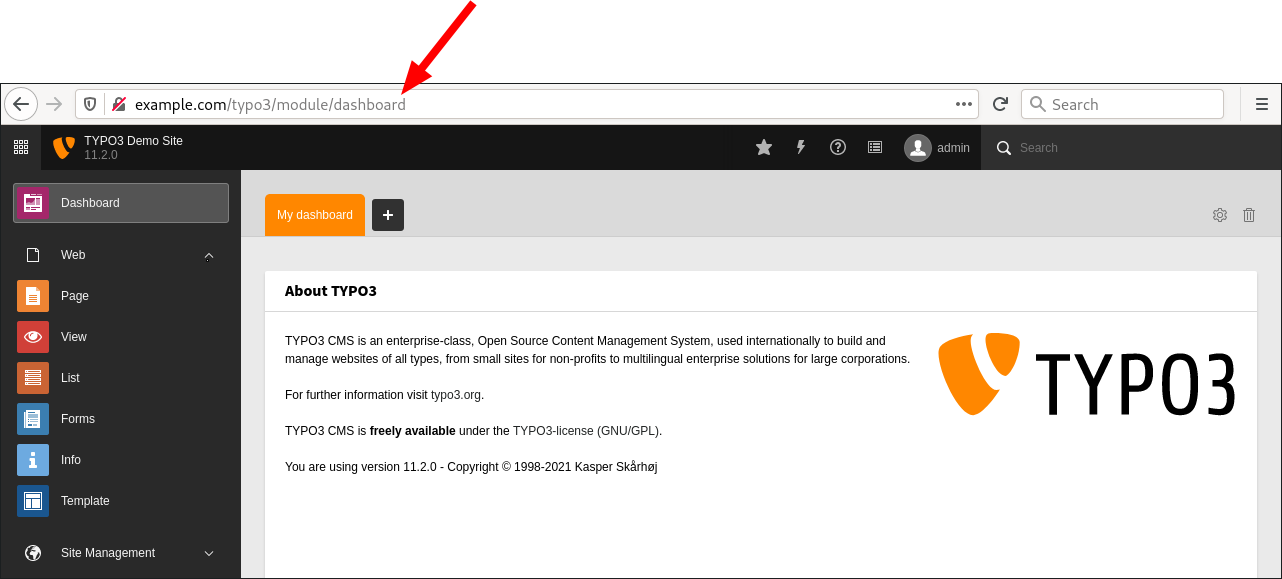
\includegraphics[width=0.85\linewidth]{BackendUserInterface/1618653909-DeepLinkingInTheBackend.png}
	\end{figure}

\end{frame}

% ------------------------------------------------------------------------------

\begin{frame}[fragile]
	\frametitle{Backend User Interface}
	\framesubtitle{Deep Linking im Backend (2)}

	Einige Beispiele für Deep Links:
	\vspace{0.2cm}
	\begin{itemize}
		\item Seiten Preview (ID=123):\newline
			\fontsize{8}{10}\texttt{https://example.com/typo3/module/web/ViewpageView?id=123}\normalsize
		\item Editieren der Site-Konfiguration:
			\fontsize{8}{10}\texttt{https://example.com/typo3/module/site/configuration?action=edit}\normalsize
		\item Bearbeitung eines Inhaltelements(ID=42):
			\fontsize{8}{10}\texttt{https://example.com/typo3/record/edit?edit[tt\_content][42]=edit}\normalsize
		\item Öffnen des Moduls "Backend Users":
			\fontsize{8}{10}\texttt{https://example.com/typo3/module/system/BeuserTxBeuser}\normalsize
	\end{itemize}

\end{frame}

% ------------------------------------------------------------------------------
